%!TEX root = index.tex
\section[Requisitos]{Requisitos}
\begin{frame}{Requisitos}
\begin{block}{Requisitos funcionais}
\begin{itemize}
	\item $20\%$ Precisão
	\item $20\%$ Abrangência
\end{itemize}
\end{block}

\begin{block}{Requisitos não funcionais}
\begin{itemize}
	\item Escalabilidade
	\item Sistema genérico
	\begin{itemize}
		\item Padronização dos dados de entrada/saída
	\end{itemize}
	\item Código aberto
\end{itemize}
\end{block}
\end{frame}

\begin{frame}{Requisitos}{Diagrama de Casos de Uso}
\begin{columns}[c]
\column{.6\textwidth}
\textbf{Três principais grupos}
	\begin{itemize}
		\item Avaliar Performance
		\item Configurar Banco de Dados
		\item Recomendar
	\end{itemize}
\column{.45\textwidth}
\begin{figure}[ht]
    \begin{center}
    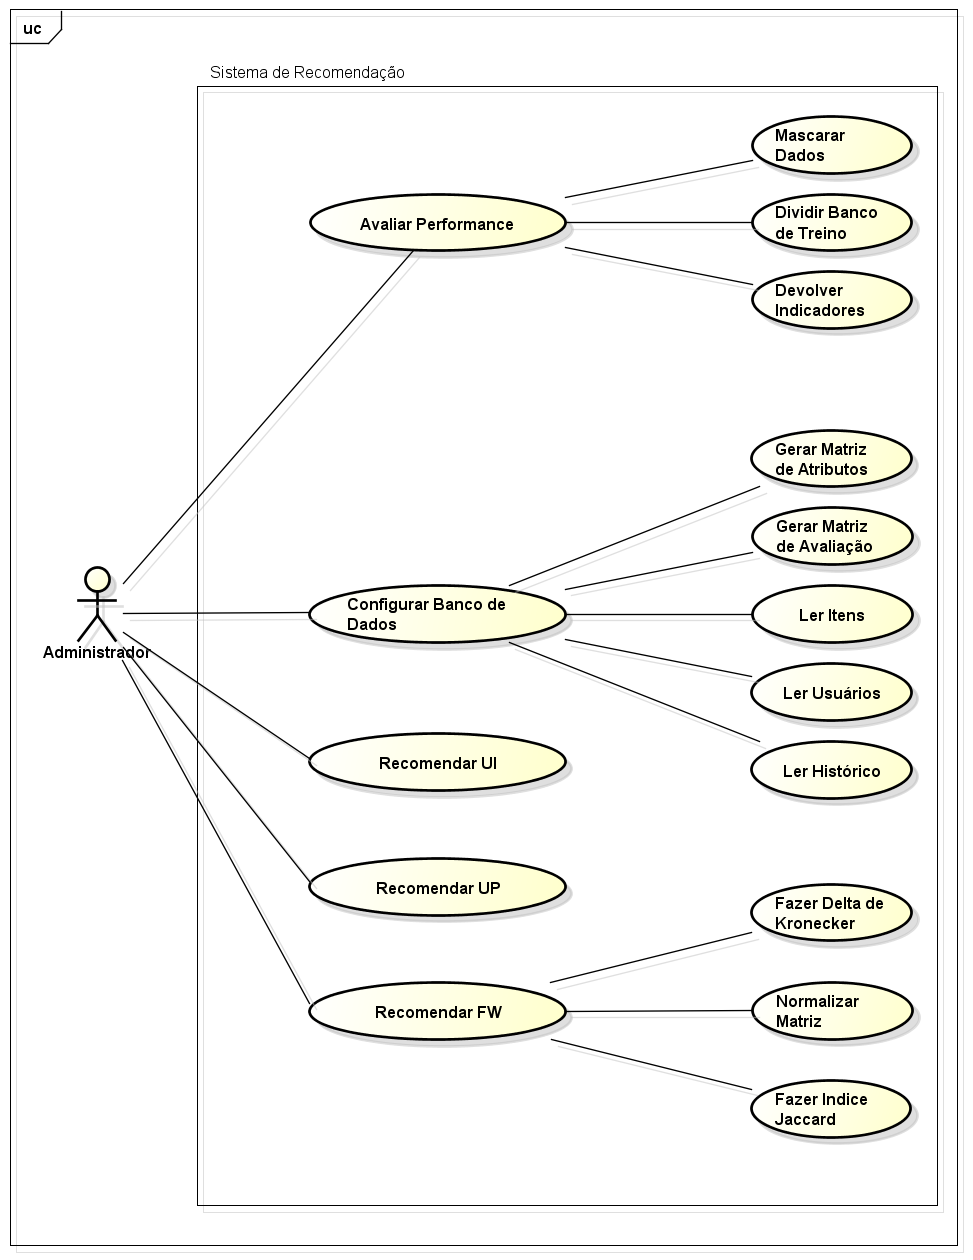
\includegraphics[width=0.9\textwidth]{img/CasosDeUso}
    \end{center}
\caption{Diagrama de Casos de Uso}
\end{figure}
\end{columns}
\end{frame}


\begin{frame}{Requisitos}{Diagrama de Casos de Uso - Avaliar Performance}

\begin{figure}[ht]
    \begin{center}
    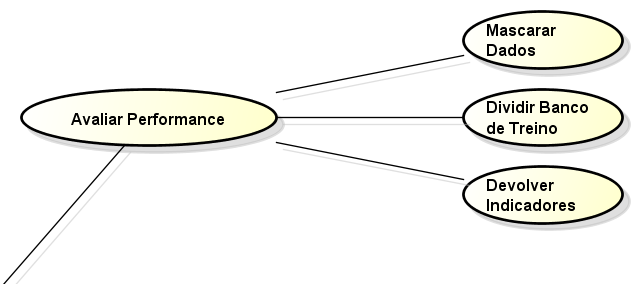
\includegraphics[width=0.9\textwidth]{img/CasosDeUso_Avaliar_Performance}
    \end{center}
\caption{Caso de Uso - Avaliar Performance}
\end{figure}
\end{frame}

\begin{frame}{Requisitos}{Diagrama de Casos de Uso - Configurar Banco de Dados}

\begin{figure}[ht]
    \begin{center}
    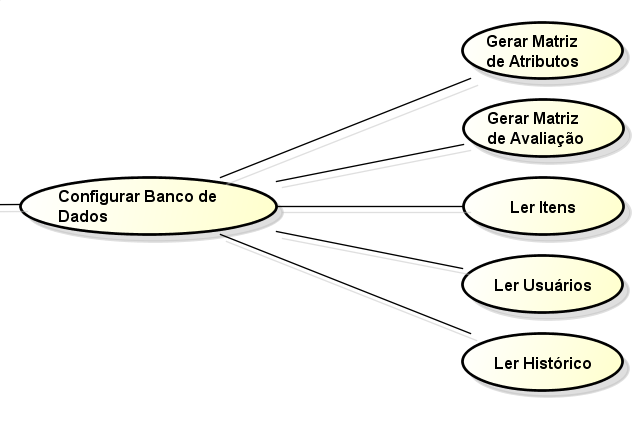
\includegraphics[width=0.9\textwidth]{img/CasosDeUso_Configurar_banco}
    \end{center}
\caption{Caso de Uso - Avaliar Performance}
\end{figure}
\end{frame}

\begin{frame}{Requisitos}{Diagrama de Casos de Uso - Recomendar}

\begin{figure}[ht]
    \begin{center}
    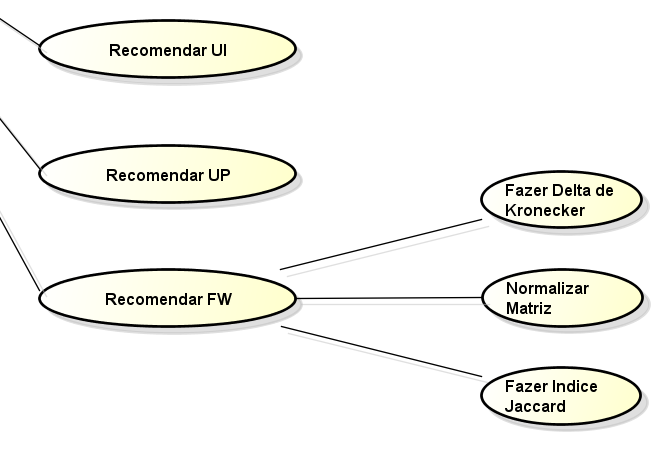
\includegraphics[width=0.9\textwidth]{img/CasosDeUso_Recomendar}
    \end{center}
\caption{Caso de Uso - Recomendar}
\end{figure}
\end{frame}